

\actTitle{Worksheet 2.1B}



\noindent \textbf{Instructions:}  Work together in groups of  3 or 4 to complete the following problems.




\begin{enumerate}

\item An object is thrown upward. The height, $h$, in feet, at time $t$, in seconds, is given by the formula $h(t) = -16t^2 + 96t$. 
\begin{enumerate}
\item Determine the number of seconds required for it to hit the ground. 
\item Determine the maximum height of the object. 
\item Determine the time required for the object to reach a height of
  50 feet on its way up.
\item For each of your steps above briefly state how the physical
  situation relates to the graph of the function $h(t)$.
\end{enumerate}

\vfill

\clearpage

\item Farmer Ed has 700 feet of fencing to enclose a rectangular plot
  that borders on a river.  If farmer Ed does not fence the side along
  the river, find the length and width of the plot that will maximize
  the area.  What is the largest area that can be enclosed?  Include
  units of measurement in your answer.

\vfill




\clearpage

\item A rectangle is drawn in the first quadrant with two sides on the
  coordinate axes and the corner opposite the origin on the line $y$ =
  $-2x+3$.  Answer the following:
  \begin{enumerate}
  \item Make a rough sketch of the situation and include all relevant
    annotations to your drawing.
  \item Write the area of the rectangle as a function of $x$.
  \item For all first quadrant points on the given line, determine the
    maximum area enclosed by the rectangle.
  \end{enumerate}

\vfill

\clearpage

\item We form two shapes using $28$ inches of string.
One shape is a square with sides of length $z$.
The other is a rectangle with width $x$ and height $3x$.
\begin{enumerate}
\item Draw a picture showing these two shapes, with their sides
  labeled, {\bf and} write a formula for the combined area $A$ of the
  two shapes.
  \sideNote{Your formula should use both $x$ and $z$ in it.}

\vspace*{1.75in}

\item We only have a small surface to work with.  Determine the
  dimensions of each shape that will minimize the combined area of
  both shapes together.
  \sideNote{Explicitly label the equation that represents the
    constraint that must be satisfied that relates $x$ and $z$.}

  \vfill

\end{enumerate}

\clearpage

\item A rectangular piece of metal has a width of eight inches, and it
  is 52 inches long. Two folds along the length of the piece will be
  made that have the same width, and when folded up the piece will
  form a gutter with a rectangular cross section and two open
  ends. Where should the folds be made so that the volume of the
  gutter will be as large as possible?

    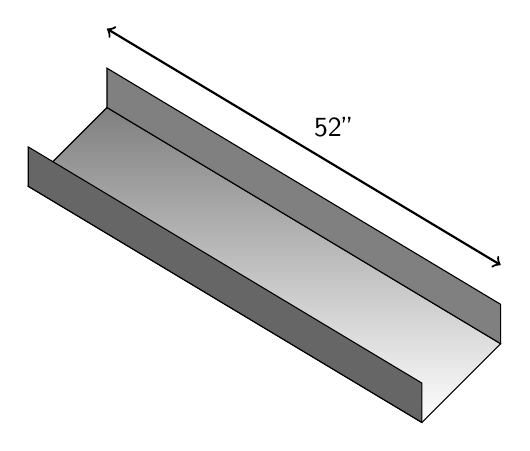
\begin{tikzpicture}[y=1.0cm, x=1.0cm,font=\sffamily]
      \path[shade,draw] (0,0) -- (5,-3) -- (6,-2) -- (1,1) -- cycle;
      \path[fill=black!50!white,draw] (1,1) -- (6,-2) -- (6,-1.5) -- (1,1.5) -- cycle;
      \path[fill=black!60!white,draw] (0,0) -- (5,-3) -- (5,-2.5) -- (0,0.5) -- cycle;
      \draw[thick,black,<->] (1,2) -- (6,-1) node[above,align=center,midway,anchor=south west] {52''};
    \end{tikzpicture}

    \vfill


\end{enumerate}


\hwTitle{Section 2.1B}

\begin{enumerate}
\item Determine two numbers whose sum is fifteen whose product is as
  large as possible.
  
\item A farmer wants to build a rectangular pen along a straight
  river.  She wants to divide the pen into 5 equal rectangular pieces
  as shown in the picture.  What is the largest area she can enclose
  with 3,000 feet of fencing?

\begin{center}
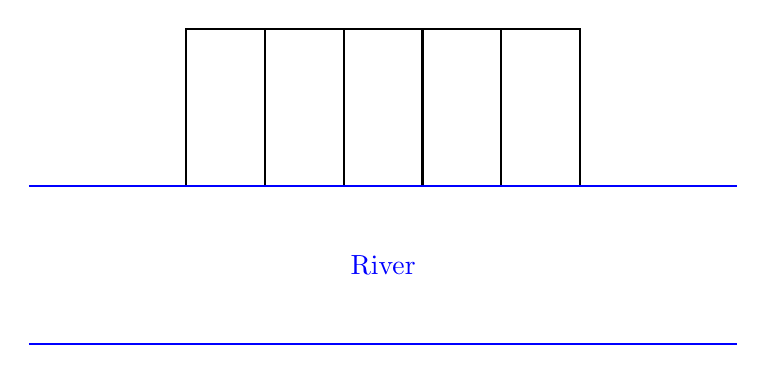
\begin{tikzpicture}[y=1.0cm, x=1.0cm]
\draw[thick] (0,0) -- (5,0) -- (5,2) -- (0, 2) -- (0,0);
\draw[thick] (1,0) -- (1,2);
\draw[thick] (2,0) -- (2,2);
\draw[thick] (3,0) -- (3,2);
\draw[thick] (4,0) -- (4,2);
\draw[thick, blue] (-2,0) -- (7,0);
\draw[thick, blue] (-2,-2) -- (7,-2);
\draw[blue] (2.5,-1) node  {River};
\end{tikzpicture}	
\end{center}


\item A Farmer will construct a rectangular pen. The pen will be
  divided into two equal parts by running a small fence North/South
  across the middle of the rectangle. What dimensions will result in a
  pen with the largest possible area?

\item A farmer will construct a rectangular pen.  The pen will be
  divided into three equal parts by running two small fences
  North/South across the middle of the rectangle.  The cost of fencing
  is eight dollars per meter, and the farmer will spend two-thousand
  dollars on fencing. What dimensions will result in a pen with the
  largest possible area?

\item A diver jumps vertically off a diving board at time $t = 0$. The
  diver's height $h$ above the water (in feet), $t$ seconds later is
  given by the formula $h(t) = -16t^2 + 6t + 5$.
\begin{enumerate}
\item Determine the number of seconds t required for the diver to reach the water ($h$ = 0)
\item How many seconds after jumping is the diver at her maximum height above the water?
\item Determine the height of the diving board above the water.
\end{enumerate}

\item There are 12 hours of daylight available to a
  bird. Suppose, the bird only takes part in two activities, foraging
  and defending its territory. The bird will fill the whole 12 hours
  with only those two activities, and each activity has an energy cost
  associated with it:
  \begin{description}
  \item[Foraging] The energy cost of foraging is 7 times the amount of
    time (in hours) spent foraging (i.e. $7*$time foraging). For
    example, if the bird spends 3 hours foraging the energy cost is 21
    energy units.
  \item[Defending Territory] To defend its territory the bird must fly
    around a large area, and the energy cost of defending its
    territory is the square of the time spent defending its territory
    (i.e. $(\mathrm{time~defending})^2$). For example, if the bird
    spends three hours defending its territory, the cost is 9 units.
  \end{description}
  
  Determine the amount of time the bird should spend foraging and the
  time defending its territory that will \textbf{minimize} the bird's
  total energy cost.


\item Farmer Brown has 400 yards of fencing with which to build a
  rectangular corral. He wants to divide it evenly into three pens, so
  he adds in two divider fences, as shown below. Answer the following:

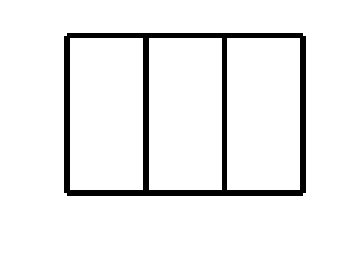
\begin{tikzpicture}[x=1.0cm,y=1.0cm]
\clip(0.5,1.5) rectangle (4.1,4.1);
\draw [line width=2.pt] (1.,4.)-- (1.,2.);
\draw [line width=2.pt] (2.,4.)-- (2.,2.);
\draw [line width=2.pt] (3.,4.)-- (3.,2.);
\draw [line width=2.pt] (4.,4.)-- (4.,2.);
\draw [line width=2.pt] (1.,4.)-- (4.,4.);
\draw [line width=2.pt] (1.,2.)-- (4.,2.);
\end{tikzpicture}

\begin{enumerate}
\item Write the area of the corral as a function of $x$: 
\item Determine the maximum area enclosed by the corral.
\end{enumerate}

\vfill

  
\end{enumerate}
